\documentclass{standalone}
\usepackage{tikz}
\usetikzlibrary{patterns, positioning}


\begin{document}
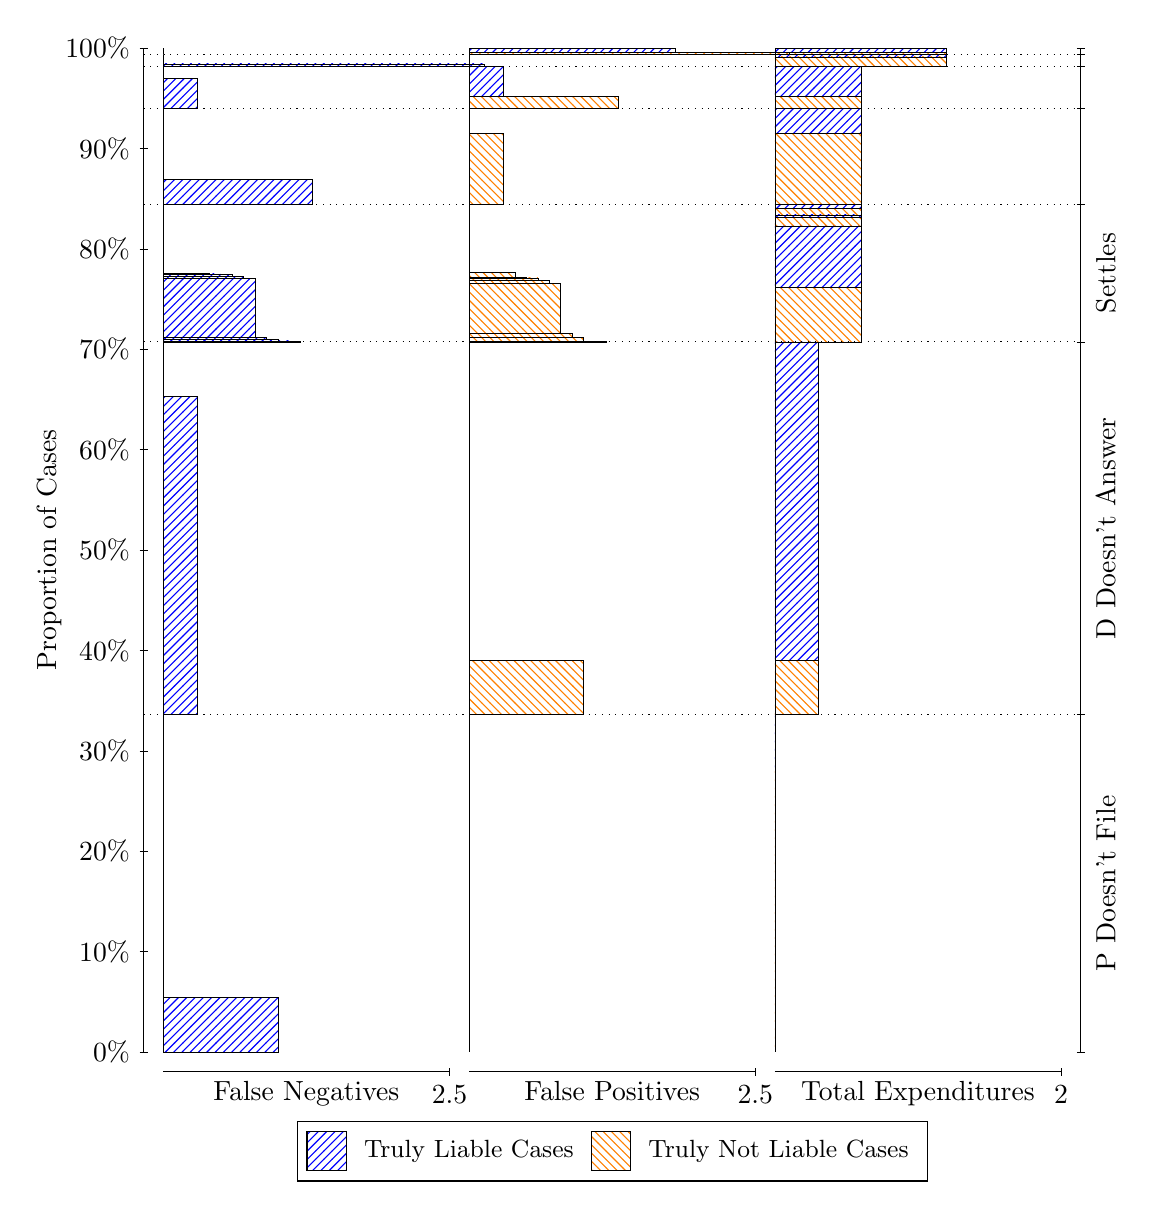
\begin{tikzpicture}
\draw[black, very thin] (1.5,1.75) -- (1.5,14.5);
\node[rotate=90, text=black, anchor=center] at (0.3, 8.125) {Proportion of Cases};
\draw[black, very thin] (1.45,1.75) -- (1.55,1.75);
\node[text=black, anchor=east] at (1.45, 1.75) {0\%};
\draw[black, very thin] (1.45,3.025) -- (1.55,3.025);
\node[text=black, anchor=east] at (1.45, 3.025) {10\%};
\draw[black, very thin] (1.45,4.3) -- (1.55,4.3);
\node[text=black, anchor=east] at (1.45, 4.3) {20\%};
\draw[black, very thin] (1.45,5.575) -- (1.55,5.575);
\node[text=black, anchor=east] at (1.45, 5.575) {30\%};
\draw[black, very thin] (1.45,6.85) -- (1.55,6.85);
\node[text=black, anchor=east] at (1.45, 6.85) {40\%};
\draw[black, very thin] (1.45,8.125) -- (1.55,8.125);
\node[text=black, anchor=east] at (1.45, 8.125) {50\%};
\draw[black, very thin] (1.45,9.4) -- (1.55,9.4);
\node[text=black, anchor=east] at (1.45, 9.4) {60\%};
\draw[black, very thin] (1.45,10.675) -- (1.55,10.675);
\node[text=black, anchor=east] at (1.45, 10.675) {70\%};
\draw[black, very thin] (1.45,11.95) -- (1.55,11.95);
\node[text=black, anchor=east] at (1.45, 11.95) {80\%};
\draw[black, very thin] (1.45,13.225) -- (1.55,13.225);
\node[text=black, anchor=east] at (1.45, 13.225) {90\%};
\draw[black, very thin] (1.45,14.5) -- (1.55,14.5);
\node[text=black, anchor=east] at (1.45, 14.5) {100\%};

\draw[black, very thin] (13.4,1.75) -- (13.4,14.5);
\draw[black, very thin] (13.35,1.75) -- (13.45,1.75);
\node[anchor=west] at (13.35, 1.75) {};
\draw[black, very thin] (13.35,6.0339) -- (13.45,6.0339);
\node[anchor=west] at (13.35, 6.0339) {};
\draw[black, very thin] (13.35,10.768) -- (13.45,10.768);
\node[anchor=west] at (13.35, 10.768) {};
\draw[black, very thin] (13.35,12.517) -- (13.45,12.517);
\node[anchor=west] at (13.35, 12.517) {};
\draw[black, very thin] (13.35,13.734) -- (13.45,13.734);
\node[anchor=west] at (13.35, 13.734) {};
\draw[black, very thin] (13.35,14.268) -- (13.45,14.268);
\node[anchor=west] at (13.35, 14.268) {};
\draw[black, very thin] (13.35,14.418) -- (13.45,14.418);
\node[anchor=west] at (13.35, 14.418) {};
\draw[black, very thin] (13.35,14.5) -- (13.45,14.5);
\node[anchor=west] at (13.35, 14.5) {};

\draw[black, very thin, pattern color=blue, pattern=north east lines] (1.75,1.75) rectangle (3.2033,2.4407);
\draw[black, very thin, pattern color=orange, pattern=north west lines] (1.75,2.4407) rectangle (1.75,6.0339);
\draw[black, very thin, pattern color=blue, pattern=north east lines] (1.75,6.0339) rectangle (2.186,10.074);
\draw[black, very thin, pattern color=orange, pattern=north west lines] (1.75,10.074) rectangle (1.75,10.768);
\draw[black, very thin, pattern color=blue, pattern=north east lines] (1.75,10.768) rectangle (3.494,10.779);
\draw[black, very thin, pattern color=blue, pattern=north east lines] (1.75,10.779) rectangle (3.3487,10.78);
\draw[black, very thin, pattern color=blue, pattern=north east lines] (1.75,10.78) rectangle (3.2033,10.802);
\draw[black, very thin, pattern color=blue, pattern=north east lines] (1.75,10.802) rectangle (3.058,10.803);
\draw[black, very thin, pattern color=blue, pattern=north east lines] (1.75,10.803) rectangle (3.058,10.824);
\draw[black, very thin, pattern color=blue, pattern=north east lines] (1.75,10.824) rectangle (2.9127,11.579);
\draw[black, very thin, pattern color=blue, pattern=north east lines] (1.75,11.579) rectangle (2.7673,11.604);
\draw[black, very thin, pattern color=blue, pattern=north east lines] (1.75,11.604) rectangle (2.622,11.63);
\draw[black, very thin, pattern color=blue, pattern=north east lines] (1.75,11.63) rectangle (2.4767,11.632);
\draw[black, very thin, pattern color=blue, pattern=north east lines] (1.75,11.632) rectangle (2.3313,11.637);
\draw[black, very thin, pattern color=orange, pattern=north west lines] (1.75,11.637) rectangle (1.75,12.517);
\draw[black, very thin, pattern color=blue, pattern=north east lines] (1.75,12.517) rectangle (3.6393,12.831);
\draw[black, very thin, pattern color=orange, pattern=north west lines] (1.75,12.831) rectangle (1.75,13.734);
\draw[black, very thin, pattern color=blue, pattern=north east lines] (1.75,13.734) rectangle (2.186,14.111);
\draw[black, very thin, pattern color=orange, pattern=north west lines] (1.75,14.111) rectangle (1.75,14.268);
\draw[black, very thin, pattern color=blue, pattern=north east lines] (1.75,14.268) rectangle (5.8193,14.298);
\draw[black, very thin, pattern color=orange, pattern=north west lines] (1.75,14.298) rectangle (1.75,14.418);
\draw[black, very thin, pattern color=orange, pattern=north west lines] (1.75,14.418) rectangle (1.75,14.448);
\draw[black, very thin, pattern color=blue, pattern=north east lines] (1.75,14.448) rectangle (1.75,14.5);
\draw[black, very thin, pattern color=orange, pattern=north west lines] (5.6333,1.75) rectangle (5.6333,5.3432);
\draw[black, very thin, pattern color=blue, pattern=north east lines] (5.6333,5.3432) rectangle (5.6333,6.0339);
\draw[black, very thin, pattern color=orange, pattern=north west lines] (5.6333,6.0339) rectangle (7.0867,6.7274);
\draw[black, very thin, pattern color=blue, pattern=north east lines] (5.6333,6.7274) rectangle (5.6333,10.768);
\draw[black, very thin, pattern color=orange, pattern=north west lines] (5.6333,10.768) rectangle (7.3773,10.773);
\draw[black, very thin, pattern color=orange, pattern=north west lines] (5.6333,10.773) rectangle (7.232,10.776);
\draw[black, very thin, pattern color=orange, pattern=north west lines] (5.6333,10.776) rectangle (7.0867,10.826);
\draw[black, very thin, pattern color=orange, pattern=north west lines] (5.6333,10.826) rectangle (6.9413,10.874);
\draw[black, very thin, pattern color=orange, pattern=north west lines] (5.6333,10.874) rectangle (6.796,11.511);
\draw[black, very thin, pattern color=orange, pattern=north west lines] (5.6333,11.511) rectangle (6.6507,11.546);
\draw[black, very thin, pattern color=orange, pattern=north west lines] (5.6333,11.546) rectangle (6.5053,11.581);
\draw[black, very thin, pattern color=orange, pattern=north west lines] (5.6333,11.581) rectangle (6.36,11.585);
\draw[black, very thin, pattern color=orange, pattern=north west lines] (5.6333,11.585) rectangle (6.2147,11.648);
\draw[black, very thin, pattern color=blue, pattern=north east lines] (5.6333,11.648) rectangle (5.924,11.653);
\draw[black, very thin, pattern color=blue, pattern=north east lines] (5.6333,11.653) rectangle (5.7787,11.655);
\draw[black, very thin, pattern color=blue, pattern=north east lines] (5.6333,11.655) rectangle (5.6333,12.517);
\draw[black, very thin, pattern color=orange, pattern=north west lines] (5.6333,12.517) rectangle (6.0693,13.42);
\draw[black, very thin, pattern color=blue, pattern=north east lines] (5.6333,13.42) rectangle (5.6333,13.734);
\draw[black, very thin, pattern color=orange, pattern=north west lines] (5.6333,13.734) rectangle (7.5227,13.89);
\draw[black, very thin, pattern color=blue, pattern=north east lines] (5.6333,13.89) rectangle (6.0693,14.268);
\draw[black, very thin, pattern color=orange, pattern=north west lines] (5.6333,14.268) rectangle (5.6333,14.387);
\draw[black, very thin, pattern color=blue, pattern=north east lines] (5.6333,14.387) rectangle (5.6333,14.418);
\draw[black, very thin, pattern color=orange, pattern=north west lines] (5.6333,14.418) rectangle (9.7027,14.448);
\draw[black, very thin, pattern color=blue, pattern=north east lines] (5.6333,14.448) rectangle (8.2493,14.5);
\draw[black, very thin, pattern color=orange, pattern=north west lines] (9.5167,1.75) rectangle (9.5167,5.3432);
\draw[black, very thin, pattern color=blue, pattern=north east lines] (9.5167,5.3432) rectangle (9.5167,6.0339);
\draw[black, very thin, pattern color=orange, pattern=north west lines] (9.5167,6.0339) rectangle (10.062,6.7274);
\draw[black, very thin, pattern color=blue, pattern=north east lines] (9.5167,6.7274) rectangle (10.062,10.768);
\draw[black, very thin, pattern color=orange, pattern=north west lines] (9.5167,10.768) rectangle (10.607,11.458);
\draw[black, very thin, pattern color=blue, pattern=north east lines] (9.5167,11.458) rectangle (10.607,12.242);
\draw[black, very thin, pattern color=orange, pattern=north west lines] (9.5167,12.242) rectangle (10.607,12.346);
\draw[black, very thin, pattern color=blue, pattern=north east lines] (9.5167,12.346) rectangle (10.607,12.382);
\draw[black, very thin, pattern color=orange, pattern=north west lines] (9.5167,12.382) rectangle (10.607,12.466);
\draw[black, very thin, pattern color=blue, pattern=north east lines] (9.5167,12.466) rectangle (10.607,12.517);
\draw[black, very thin, pattern color=orange, pattern=north west lines] (9.5167,12.517) rectangle (10.607,13.42);
\draw[black, very thin, pattern color=blue, pattern=north east lines] (9.5167,13.42) rectangle (10.607,13.734);
\draw[black, very thin, pattern color=orange, pattern=north west lines] (9.5167,13.734) rectangle (10.607,13.89);
\draw[black, very thin, pattern color=blue, pattern=north east lines] (9.5167,13.89) rectangle (10.607,14.268);
\draw[black, very thin, pattern color=orange, pattern=north west lines] (9.5167,14.268) rectangle (11.697,14.387);
\draw[black, very thin, pattern color=blue, pattern=north east lines] (9.5167,14.387) rectangle (11.697,14.418);
\draw[black, very thin, pattern color=orange, pattern=north west lines] (9.5167,14.418) rectangle (11.697,14.448);
\draw[black, very thin, pattern color=blue, pattern=north east lines] (9.5167,14.448) rectangle (11.697,14.5);
\draw[black, dotted] (1.5,6.0339) -- (13.4,6.0339);
\draw[black, dotted] (1.5,10.768) -- (13.4,10.768);
\draw[black, dotted] (1.5,12.517) -- (13.4,12.517);
\draw[black, dotted] (1.5,13.734) -- (13.4,13.734);
\draw[black, dotted] (1.5,14.268) -- (13.4,14.268);
\draw[black, dotted] (1.5,14.418) -- (13.4,14.418);
\draw[black, very thin] (1.75,1.5) -- (5.3833,1.5);
\node[text=black, anchor=north] at (3.5667, 1.5) {False Negatives};
\draw[black, very thin] (5.3833,1.45) -- (5.3833,1.55);
\node[text=black, anchor=north] at (5.3833, 1.45) {2.5};

\draw[black, very thin] (5.6333,1.5) -- (9.2667,1.5);
\node[text=black, anchor=north] at (7.45, 1.5) {False Positives};
\draw[black, very thin] (9.2667,1.45) -- (9.2667,1.55);
\node[text=black, anchor=north] at (9.2667, 1.45) {2.5};

\draw[black, very thin] (9.5167,1.5) -- (13.15,1.5);
\node[text=black, anchor=north] at (11.333, 1.5) {Total Expenditures};
\draw[black, very thin] (13.15,1.45) -- (13.15,1.55);
\node[text=black, anchor=north] at (13.15, 1.45) {2};

\node[text=black, centered, rotate=90] at (13.72, 3.892) {P Doesn't File};
\node[text=black, centered, rotate=90] at (13.72, 8.4008) {D Doesn't Answer};
\node[text=black, centered, rotate=90] at (13.72, 11.642) {Settles};





\draw (7.449999999999999,1.5) node[draw=none] (baseCoordinate) {};
\begin{scope}[align=center]
        \matrix[scale=0.5, draw=black, below=0.5cm of baseCoordinate, nodes={draw}, column sep=0.1cm]{
            \node[rectangle, draw, minimum width=0.5cm, minimum height=0.5cm, pattern color=blue, pattern=north east lines] {}; &
            \node[draw=none, font=\small, text=black] (B) {Truly Liable Cases}; &
            \node[rectangle, draw, minimum width=0.5cm, minimum height=0.5cm, pattern color=orange, pattern=north west lines] {}; &
            \node[draw=none, font=\small, text=black] (B) {Truly Not Liable Cases}; \\
            };
\end{scope}

\end{tikzpicture}
\end{document}